\documentclass[11pt, a4paper]{article}
\usepackage{graphicx}
\usepackage{amsmath}
\usepackage{listings}
\usepackage{mathrsfs}



\title{Assignment 7} % Title

\author{Om Shri Prasath (EE17B113)} % Author name

\date{\today} % Date for the report
\begin{document}	

\maketitle % Insert the title, author and date
\section{Introduction}\label{introduction}

\begin{itemize}
\item
  We analyse the LTI systems in continuous time using Laplace
  transform to find the solutions to the equations governing the system
  with the help of python tools such as Symbolic python known as
  \(Sympy\) and Signal toolbox.\\
\item
  $symbols \to $ used to declare symbols using sympy.
\item
  $lambdify \to $ Converts the sympy expression into one numpy
  expression which can be evaluated.
\item
  \(system.impulse \to\) Computes the impulse response of the transfer
  function
\item
  \(sp.lti \to\) defines a transfer function from polynomial
  coefficients of numerator and denominator as inputs.
\item
  In this assignment we solve all equations analytically using
  expressions with variables like we use to solve manually with
  variables which is unlike the way we generally follow to solve i.e by
  solving for some specific cases (Numerically)) rather than solving for
  general case with variables.
\item
  So we use Symbolic python to do the above mentioned and we analyse the
  circuits by solving them analytically and analyse the systems finally
  using numpy.
\end{itemize}   
\newpage
\section{Python Code}\label{code}

\subsection{Question 1:}\label{question-1}

\begin{itemize}
\item
  We analyse a Low pass filter circuit given below using symbolic python
  and numpy.
\item
  Observe and analyse the responses of the systems for various inputs.
\end{itemize}

\begin{figure}[!tbh]
  \centering
  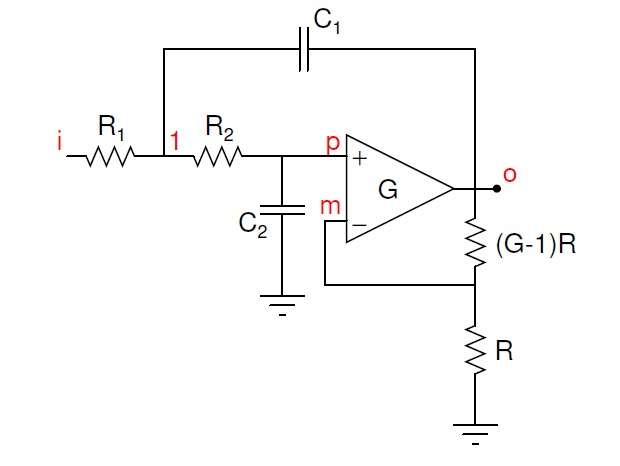
\includegraphics[scale=0.5]{./../Extras/circuit1.jpeg}  % Mention the image name within the curly braces. Image should be in the same folder as the tex file. 
      \caption{Active Lowpass Filter circuit}
\end{figure}

\begin{itemize}
\item
  Using sympy we can represent the nodal equations of the ciruit in the
  form of matrix and solve it to find Vo(t).
\end{itemize}

\[\begin{pmatrix} 0 & 0 & 1 & -\frac{1}{G} \\ -\frac{1}{1+sR2C2} & 1 & 0 & 0 \\ 0 & -G & G & 1 \\ -\frac{1}{R_1}-\frac{1}{R_2}-sC_1 & \frac{1}{R2} & 0 & sC_1 \end{pmatrix}\begin{pmatrix} V_1 \\ V_p \\ V_m \\ V_o \end{pmatrix} = \begin{pmatrix} 0 \\ 0 \\ 0 \\ -V_i(s)/R_1 \end{pmatrix}\]

\begin{itemize}
\item
  Obtain the Transfer function of the network, which is determined by
  finding laplace transform of impulse response
  (\(V_{i}(t) = \delta (t)\) whose \(Laplace \ Transform\) is
  \(\mathcal{V}_i(s) = \frac{1}{s}\)).
\item
  From transfer function obtain the Quality factor of the system, which
  essentially says how sharp the system is certain range frequencies.
\item
  If \(Q < 0.5\) system is overdamped since damping factor
  \(\zeta = \frac{1}{2Q} > 1\) for \(Q<0.5\) which means the unit step
  response will raise slowly from 0 to \(V_{max}\) exponentially unlike
  immediately changing from \(0 \ to V_{max}\).
\item
  To observe this behaviour we give unit step as input and analyse the
  output.
\item
  Obtain unit step response of the system i.e
\end{itemize}

\begin{equation}
V_{i}(t) = u(t) \ Volts
\end{equation}

\begin{equation}
\mathcal{V}_{i}(s) = \frac{1}{s}
\end{equation}

\begin{itemize}
\item
  Obtain and analyse the response for sinusoid with a low frequency and
  high frequency component of
  \(\omega_1 = 2000\pi \ rads^{-1} \ and \ \omega_2 = 2*10^{6}\pi \ rads^{-1}\).
\end{itemize}

\begin{equation}
V_{i}(t) = ( \ \sin(2000\pi t) + \cos(2*10^{6}\pi t) \ )u_{o}(t) \ Volts
\end{equation}

\begin{itemize}
\item
  \(sp.lsim\) is used for finding the output in time domain.
\item
  Determine and Plot the output voltage \(V_{o}(t)\) for the cases above
  and analyse them.
\end{itemize}
\textit{\textbf{Code:}}
   \begin{lstlisting}
def lowpass(R1, R2, C1, C2, G, Vi):
  s = symbols('s')
  A = Matrix([[0, 0, 1, -1/G], [-1/(1+s*R2*C2), 1, 0, 0],
              [0, -G, G, 1], [-1/R1-1/R2-s*C1, 1/R2, 0, s*C1]])
  b = Matrix([0, 0, 0, Vi/R1])
  V = A.inv()*b
  return (A, b, V)

def sympytolti(n_coeff, d_coeff):
  n_coeff = np.array(n_coeff, dtype=float)
  d_coeff = np.array(d_coeff, dtype=float)
  H_n = poly1d(n_coeff)
  H_d = poly1d(d_coeff)
  Hs = sp.lti(H_n, H_d)
  return Hs


def solve_circuit(R1, R2, C1, C2, G, Vi, input_freqresponse):
  s = symbols('s')
  A, b, V = input_freqresponse(R1, R2, C1, C2, G, Vi)
  Vo = V[3]
  num, den = fraction(simplify(Vo))
  num_coeffs = Poly(num, s).all_coeffs()
  den_coeffs = Poly(den, s).all_coeffs()
  Vlti = sympytolti(num_coeffs, den_coeffs)
  w = logspace(0, 8, 801)
  ss = 1j*w
  hf = lambdify(s, Vo, "numpy")
  v = hf(ss)

  # Calculating Quality factor for the system
  if(Vi == 1):
      # Vi(s)=1 means input is impulse
      Q = sqrt(1/(pow(den_coeffs[1]/den_coeffs[2],
                      2) / (den_coeffs[0]/den_coeffs[2])))
      print("Quality factor of the system : %g" % (Q))
      return v, Vlti, Q
  else:
      return v, Vlti


# Declaring params of the circuit1
R1 = 10000
R2 = 10000
C1 = 1e-9
C2 = 1e-9
G = 1.586
# w is x axis of bode plot
s = symbols('s')
w = logspace(0, 8, 801)
Vi_1 = 1  # Laplace transform of impulse
Vi_2 = 1/s  # Laplace transform of u(t)

# Impulse response of the circuit
Vo1, Vs1, Q = solve_circuit(R1, R2, C1, C2, G, Vi_1, lowpass)
# To find Output Voltage in time domain
t1, Vot1 = sp.impulse(Vs1, None, linspace(0, 1e-2, 10000))
# Step response of circuit
Vo2, Vs2 = solve_circuit(R1, R2, C1, C2, G, Vi_2, lowpass)
# To find Output Voltage in time domain
t2, Vot2 = sp.impulse(Vs2, None, linspace(0, 1e-3, 10000))

# Magnitude response for impulse (in loglog)
loglog(w, abs(Vo1),
        label=r"$|H(j\omega)|$")
title(r"Figure 1a: $|H(j\omega)|$ : Magnitude response 
of Transfer function")
legend()
xlabel(r"$\omega \to $")
ylabel(r"$ |H(j\omega)| \to $")
grid()
show()

# Plot of output for step input
step([t2[0], t2[-1]], [0, 1], label=r"$V_{i}(t) = u(t)$")
plt.plot(t2, abs(Vot2), label=r"Response for $V_{i}(t) = u(t)$")
legend()
title(r"Figure 1b: $V_{o}(t)$ : Unit Step response in time domain")
xlabel(r"$t \to $")
ylabel(r"$ V_{o}(t) \to $")
grid()
show()

   \end{lstlisting}
\newpage
\begin{figure}[!tbh]
    \centering
    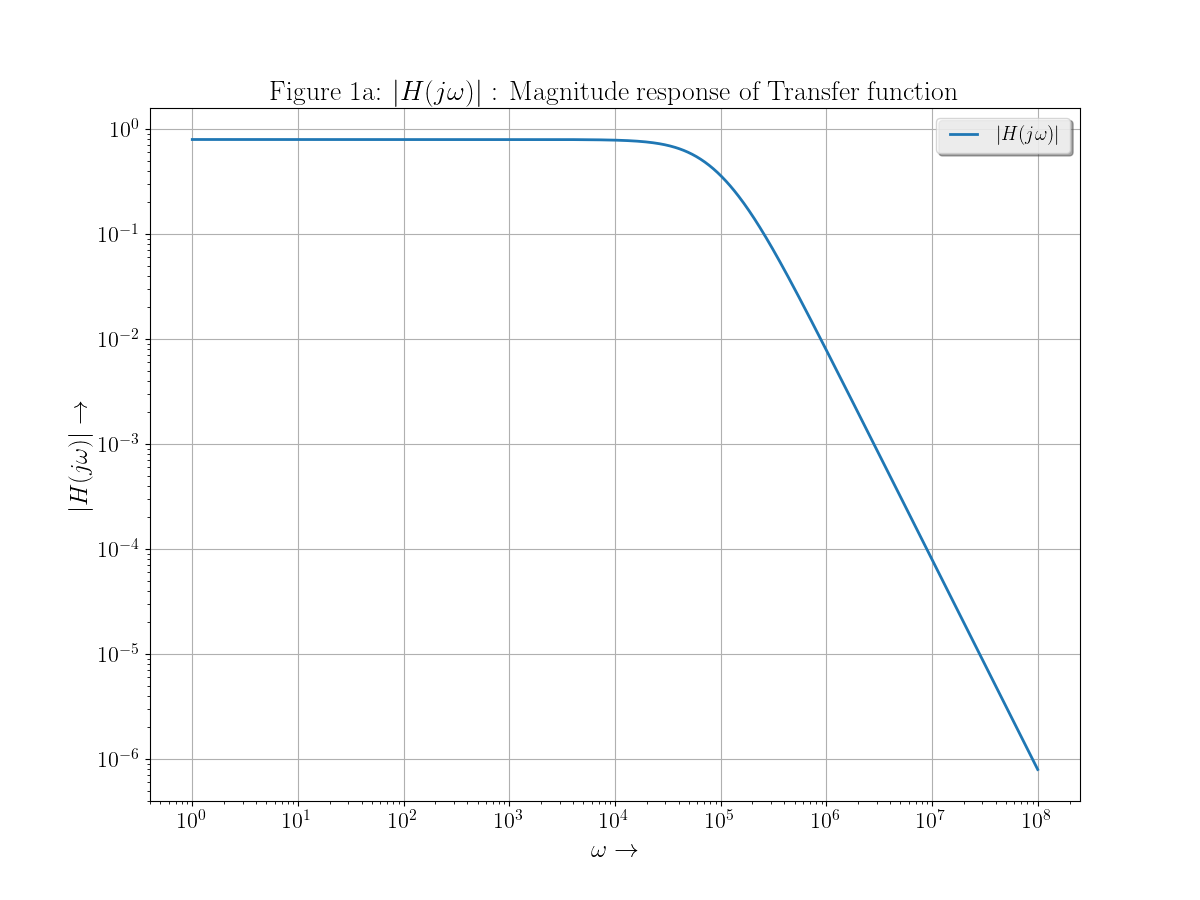
\includegraphics[scale=0.4]{./../Extras/A71a.png}  % Mention the image name within the curly braces. Image should be in the same folder as the tex file. 
    
    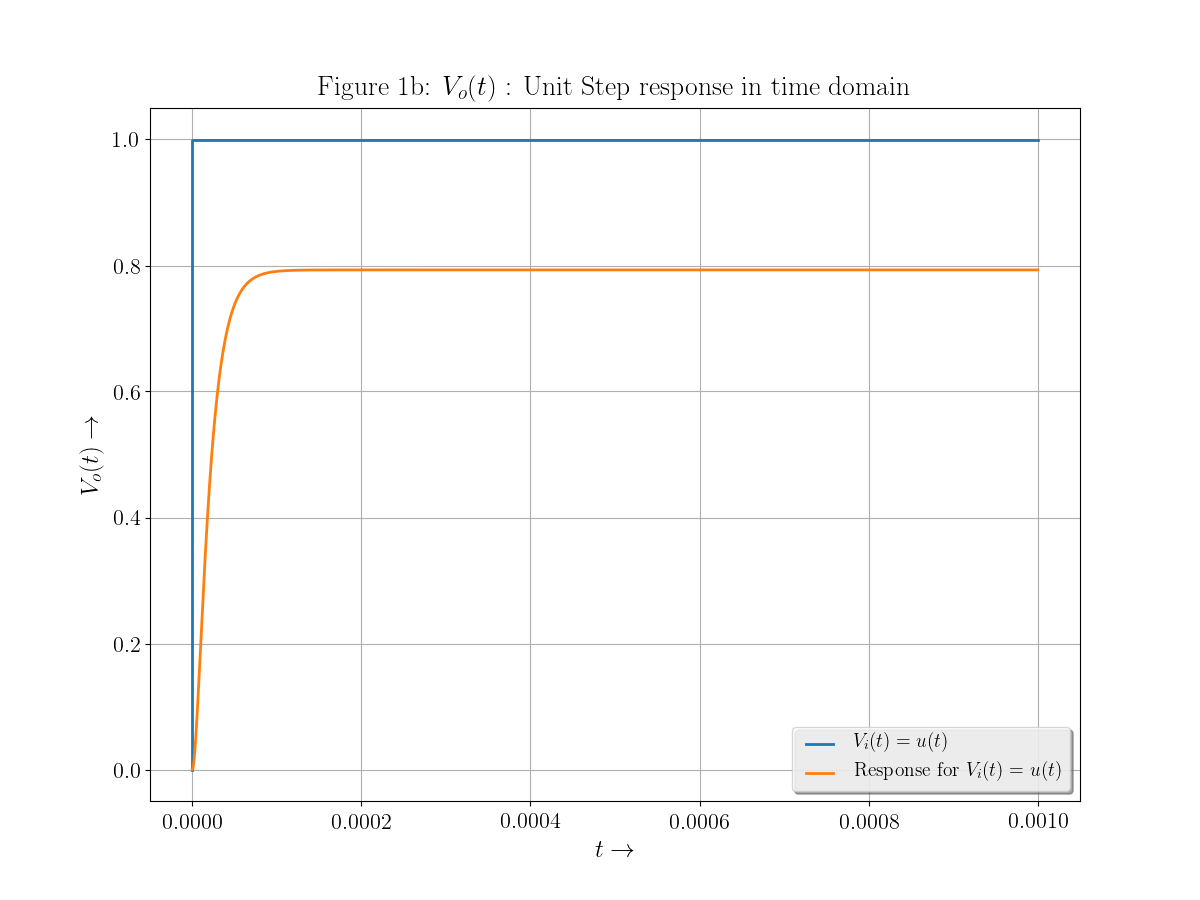
\includegraphics[scale=0.4]{./../Extras/A71b.png}  % Mention the image name within the curly braces. Image should be in the same folder as the tex file. 
    \caption{Plots of impulse response(Bode plot) and step response of circuit}
  \end{figure}
\newpage

\subsubsection{Results and Discussion:}\label{results-and-discussion}

\begin{itemize}

\item
  As we observe the Bode plot and the circuit that we know it is a low pass
  filter with bandwidth \\ $ 0 \textless{} \omega \textless{} 10^{4}$.
\item
  So the circuit will only pass input with frequencies which are in
  range of bandwidth only and attenuates other frequencies largely since
  its second order filter with -40dB/dec drop in gain
  \item
  As we observe the step response plot that \(V_{o}(t)\) increases quickly from 0 to
  0.8 and settles at 0.8 for after some time and remains constant.
\item
  Because since the network is lowpass filter, the output must be
  dominated by DC gain at steady state.
\item
  And we determined Quality factor of the system as
  \(Q = 0.453.. < \frac{1}{\sqrt{2}}\) Which implies that the gain of
  the system never exceeds DC Gain and always less than that. This
  observation comes by analysing the general form of second order
  transfer function.
\item
  So with this we see that unit step response is always less that the DC
  Gain of \(0.8\) which is obtained by putting \(s=0\) in the
  \(\mathcal{V}_{o}(s)\).
\item
  Also If \(Q < 0.5\) system is overdamped since damping factor
  \(\zeta = \frac{1}{2Q} > 1\) for \(Q<0.5\) which means the unit step
  response will raise slowly from 0 to \(V_{max}\) exponentially unlike
  immediately changing from \(0 \ to V_{max}\)
\item
  So this is also observed in the plot as it slowly raises from 0 to 0.8
  and settles.

\end{itemize}
  \newpage
  \subsection{Question 2:}\label{question-2}

  \begin{itemize}
  \item
    Now we give different input to the same circuit given above :
    \(V_{i}(t)\) as follows
  \end{itemize}
  
  \begin{equation}
  V_{i}(t) = ( \ \sin(2000\pi t) + \cos(2x10^{6}\pi t) \ )u_{o}(t) \ Volts
  \end{equation}
  
  \begin{itemize}
  \item
    Determine the output voltage \(V_{o}(t)\) using sp.lsim.
  \item
    Plot  \(V_{o}(t)\) and analyse the results.
  \end{itemize}
    \textit{\textbf{Code:}}
   \begin{lstlisting}
# Input sinusoid frequencies in rad/s
w1 = 2000*np.pi
w2 = 2*1e6*np.pi

ts = np.linspace(0, 0.005, 8001)

vi = np.sin(w1*ts)+np.cos(w2*ts)
t, Vout, svec = sp.lsim(Vs1, vi, ts)

#Plotting the output for sinusoid
plt.plot(ts, Vout, label=r"Response for $V_{i}(t) = $ Sinusoid")
legend()
title(r"Figure 2: $V_{o}(t)$ : Output Voltage for sinusoidal input")

xlabel(r"$t \to $")
ylabel(r"$ V_{o}(t) \to $")
plt.ylim([-1.1, 1.1])
grid()
show()
   \end{lstlisting}
   \newpage
   \begin{figure}[!tbh]
    \centering
    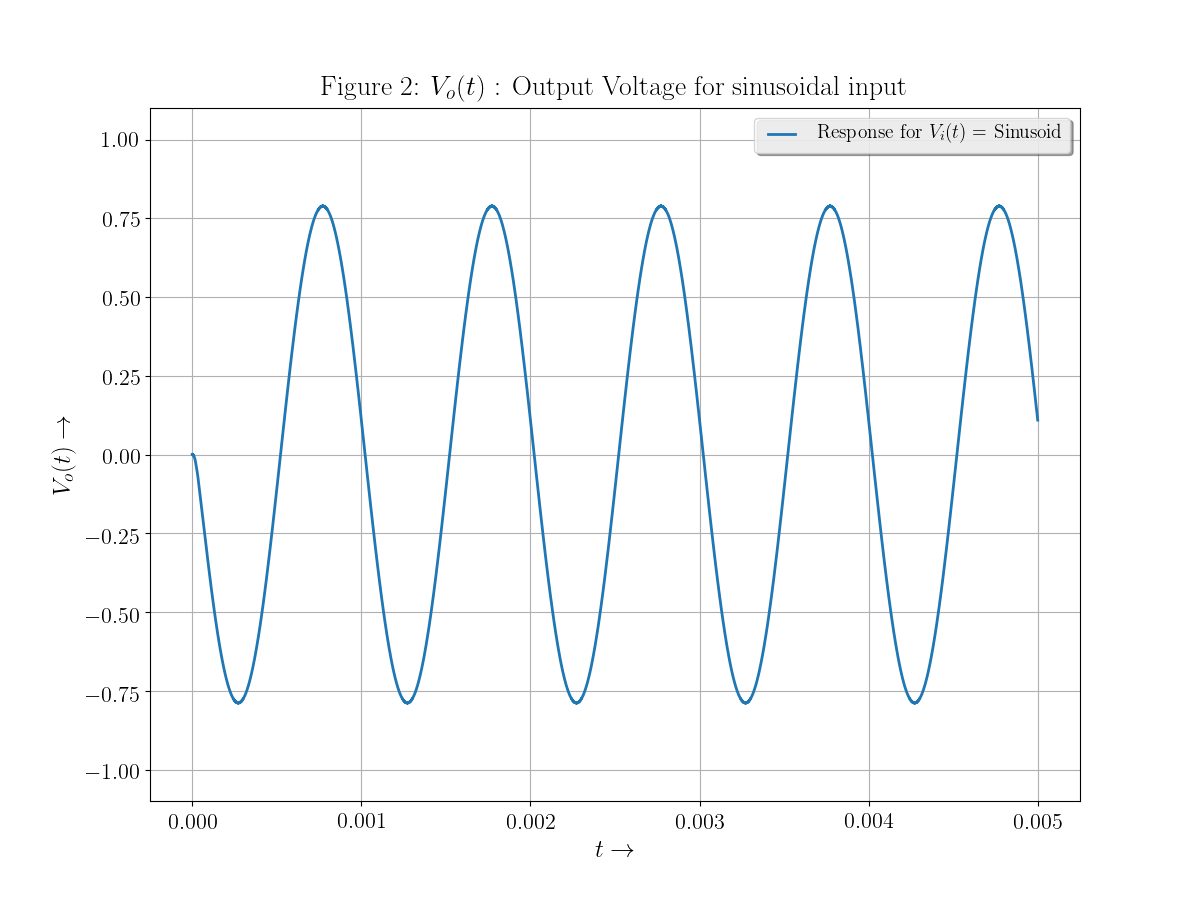
\includegraphics[scale=0.5]{./../Extras/A72.png}  % Mention the image name within the curly braces. Image should be in the same folder as the tex file. 
   \caption{Plots of sinusoid response}
  \end{figure}
  \newpage
  \subsubsection{Results and Discussion:}\label{results-and-discussion}
\begin{itemize}
  \item
  From the plot, we can see that the circuit will only pass input with frequencies which are in
  range of its bandwidth only. But since its not a ideal low pass filter as
  its gain doesn't drop abruptly at \(10^4\) rather gradual decrease
  which is observed from magnitude response plot.
\item
  So the output \(V_o(t)\) will be mainly of \(\sin(2000\pi t)\) with
  higher frequencies attenuated largely since its second order filter so
  gain drops 40dB/dec.
\item
  Since its \(\sin\) function, we can observe that \(V_{o}(t)\) starts
  from 0
\end{itemize}
\newpage
\section{Question 3 ,4 \& 5:}\label{question-3-4-5}

\begin{itemize}

\item
  Now we analyse a High pass filter circuit given below using symbolic
  python.
\item
  We will observe the responses of the systems for various inputs.
\end{itemize}

\begin{itemize}

\item
  Using sympy we can represent the nodal equations of the ciruit in the
  form of matrix and solve it to find Vo(t).
\end{itemize}

\[\begin{pmatrix} 0 & 0 & 1 & -\frac{1}{G} \\ -\frac{-sR_3C_2}{1+sR_3C_2} & 1 & 0 & 0 \\ 0 & -G & G & 1 \\ -1-(sR_1C_1)-(sR_3C_2)) & sC_2R_1 & 0 & 1 \end{pmatrix}\begin{pmatrix} V_1 \\ V_p \\ V_m \\ V_o \end{pmatrix} = \begin{pmatrix} 0 \\ 0 \\ 0 \\ -V_i(s)sR_1C_1 \end{pmatrix}\]

\begin{itemize}
\item 
	$R_1 = 10k$,$ R_2 = 10k, \ C1 = C2 = 10^{-9} F$
\end{itemize}

\begin{figure}[!h]
\centering
\  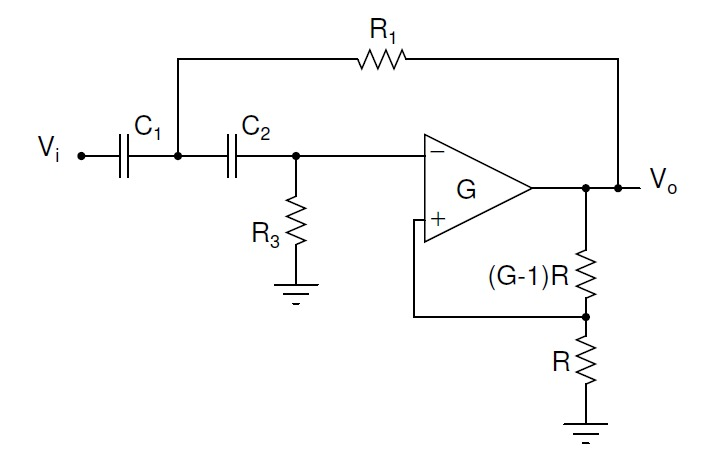
\includegraphics[scale=0.5]{./../Extras/circuit2.jpeg}  % Mention the image name within the curly braces. Image should be in the same folder as the tex file. 
\caption{Active Lowpass Filter circuit}
\end{figure}


\begin{itemize}
\item Obtain the Transfer function of the network, which is determined by
finding laplace transform of impulse response(\(V_{i}(t) = \delta t\)).
\end{itemize}


\begin{itemize}

\item
  Obtain and analyse the response for undamped and damped sinusoids.
\end{itemize}

\begin{equation}
V_{i}(t) = ( \ \sin(2000\pi t) + \cos(2x10^{6}\pi t) \ )u_{o}(t) \ Volts
\end{equation}

\begin{equation}
V_{i}(t) = e^{-10^{5}t}( \ \sin(2000\pi t) + \cos(2x10^{6}\pi t) \ )u_{o}(t) \ Volts
\end{equation}

\begin{itemize}
\item
  \(sp.lsim\) is used for finding the output in time domain
\item
  Determine and Plot the output voltage \(V_{o}(t)\) for both the cases
  above and analyse them.
\item
  Using results obtained from this network and previous network compare
  them and analyse the differences.
\end{itemize}
\textit{\textbf{Code:}}
\begin{lstlisting}
def highpass(R1, R3, C1, C2, G, Vi):
s = symbols('s')
A = Matrix([[0, 0, 1, -1/G],
            [(-s)*C2*R3/(1+s*R3*C2), 1, 0, 0],
            [0, -G, G, 1],
            [(-1-(s*R1*C1)-(s*R3*C2)), s*C2*R1, 0, 1]])
b = Matrix([0, 0, 0, -Vi*s*C1*R1])
V = A.inv()*b
return (A, b, V)

R1b = 10000
R3b = 10000
C1b = 1e-9
C2b = 1e-9
Gb = 1.586
# input frequencies for damped sinusoids
w1 = 2000*np.pi
w2 = 2e6*np.pi
# Decay factor for damped sinusoid
a = 1e5

# Laplace transform of impulse
Vi_1b = 1
# Laplace of unit step
Vi_2b = 1/s

# Solve for step response
Vo1b, Vs1b, Qb = solve_circuit(R1b, R3b, C1b, C2b, Gb, Vi_1b, highpass)
t1b, Vot1b = sp.impulse(Vs1b, None, linspace(0, 1e-2, 10000))

# Solve for impulse response
Vo2b, Vs2b = solve_circuit(R1b, R3b, C1b, C2b, Gb, Vi_2b, highpass)
t2b, Vot2b = sp.impulse(Vs2b, None, linspace(0, 5e-4, 1000001))

ts1 = np.linspace(0, 0.000005, 800001)
ts2 = np.linspace(0, 0.00003, 80001)

V_i3b = np.sin(w1*ts1)+np.cos(w2*ts1)

V_i4b = np.exp(-a*ts2)*(np.sin(w1*ts2)+np.cos(w2*ts2))

t3b, Vot3b, svec = sp.lsim(Vs1b, V_i3b, ts1)

t4b, Vot4b, svec = sp.lsim(Vs1b, V_i4b, ts2)

loglog(w, abs(Vo1b), label=r"$|H(j\omega)|$")
legend()
title(r"Figure 3a: $|H(j\omega)|$ : Magnitude response of Transfer function")
xlabel(r"$\omega \to $")
ylabel(r"$ |H(j\omega)| \to $")
grid()
show()

step([t2b[0], t2b[-1]], [0, 1], label=r"$V_{i}(t) = u(t)$")
plt.plot(t2b, Vot2b, label=r"Unit Step Response for $V_{i}(t) = u(t)$")
legend()
title(r"Figure 3b: $V_{o}(t) $ : Unit step response in time domain")
xlabel(r"$ t (seconds) \to $")
ylabel(r"$ V_{o}(t) \to $")
grid()
show()

plt.plot(t3b, (Vot3b), label=r"Response for $V_{i}(t) = $ Undamped Sinusoid")
legend()
title(r"Figure 4: $V_{o}(t)$ : Output Voltage for undamped sinusoid input")
xlabel(r"$t \to $")
ylabel(r"$ V_{o}(t) \to $")
plt.ylim([-1.1, 1.1])
grid()
show()

plt.plot(t4b, (Vot4b), label=r"Response for $V_{i}(t) = $ Damped Sinusoid")
legend()
title(r"Figure 5: $V_{o}(t)$ : Output Voltage for damped sinusoid input")
xlabel(r"$t \to $")
ylabel(r"$ V_{o}(t) \to $")
grid()
show()
\end{lstlisting}
\newpage
\begin{figure}[!tbh]
  \centering
  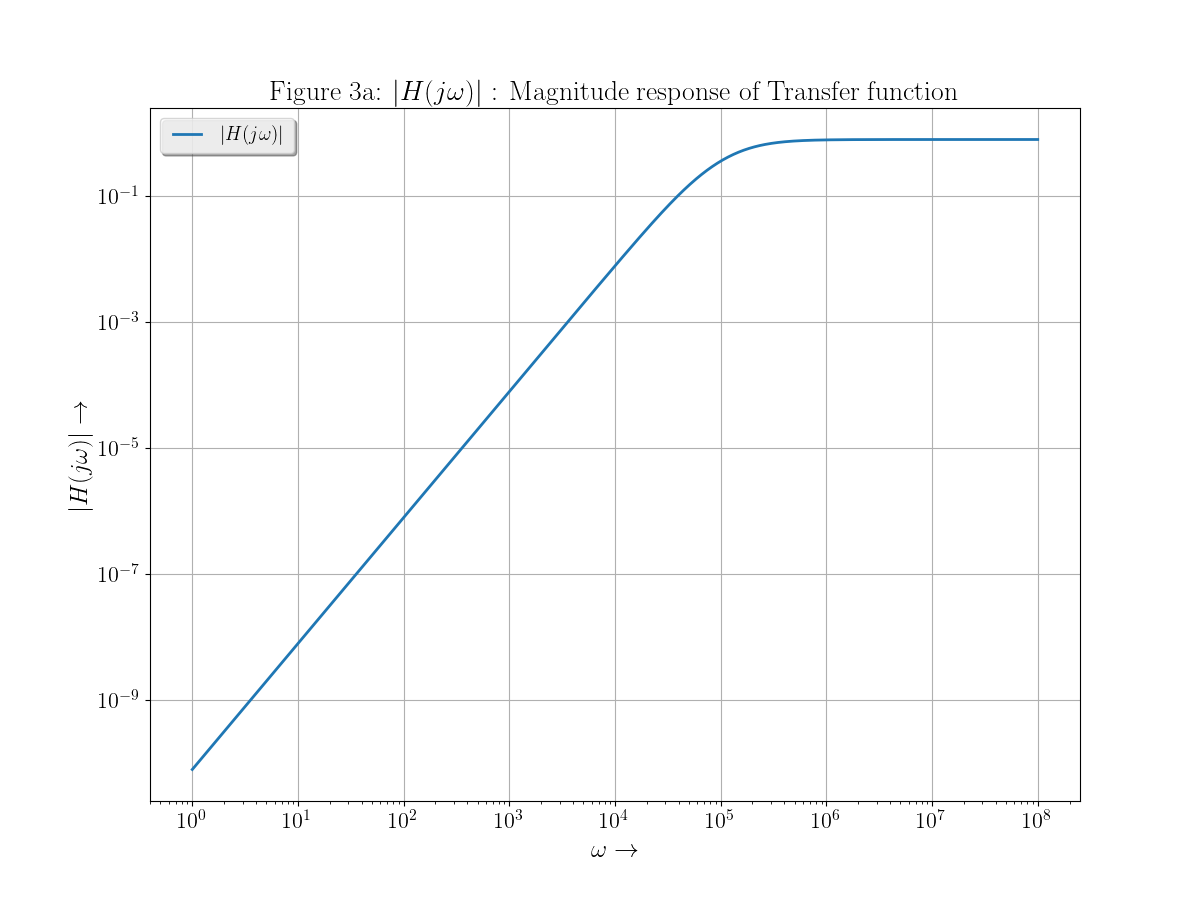
\includegraphics[scale=0.4]{./../Extras/A73a.png}  % Mention the image name within the curly braces. Image should be in the same folder as the tex file. 
  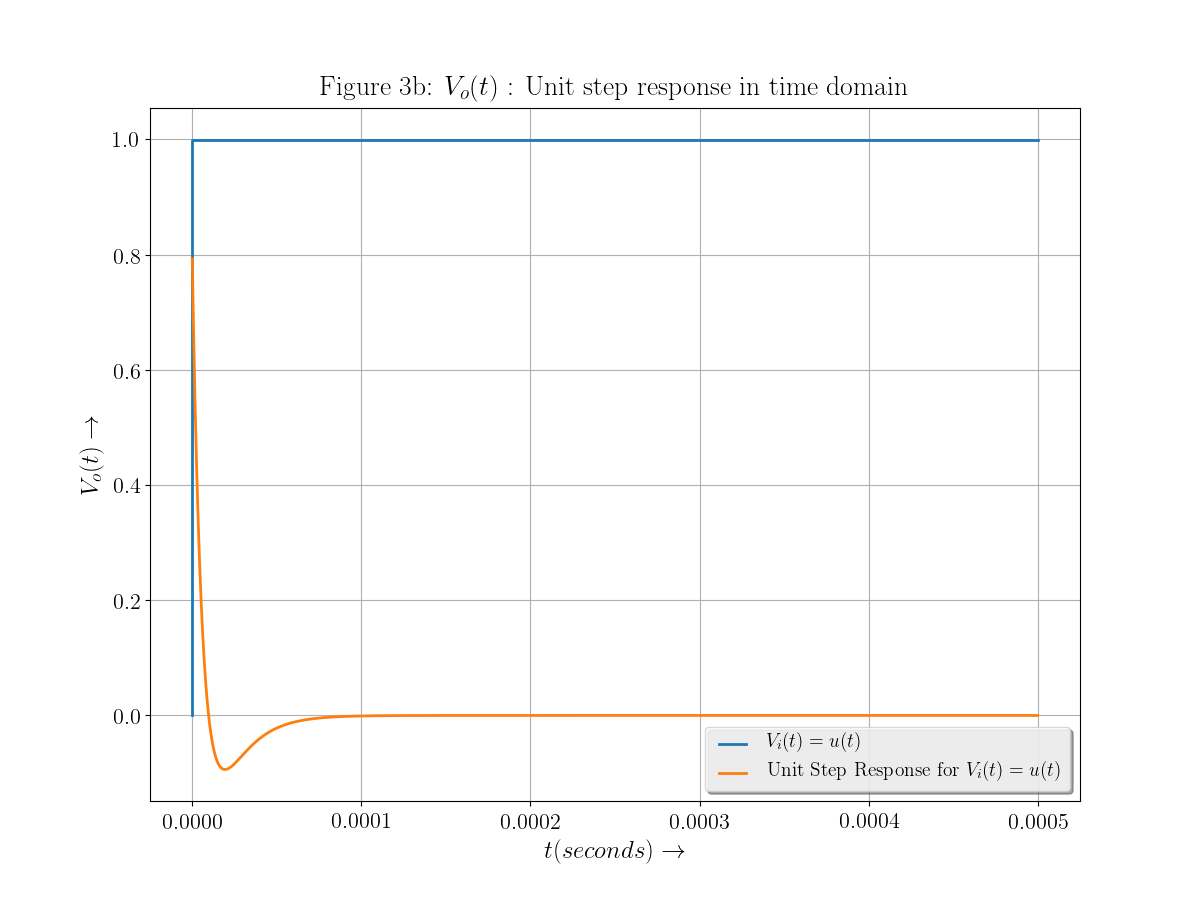
\includegraphics[scale=0.4]{./../Extras/A73b.png}  % Mention the image name within the curly braces. Image should be in the same folder as the tex file. 
 
  \caption{Plots of impulse(Bode plot) and step response}
\end{figure}

\newpage

\begin{figure}[!tbh]
  \centering
  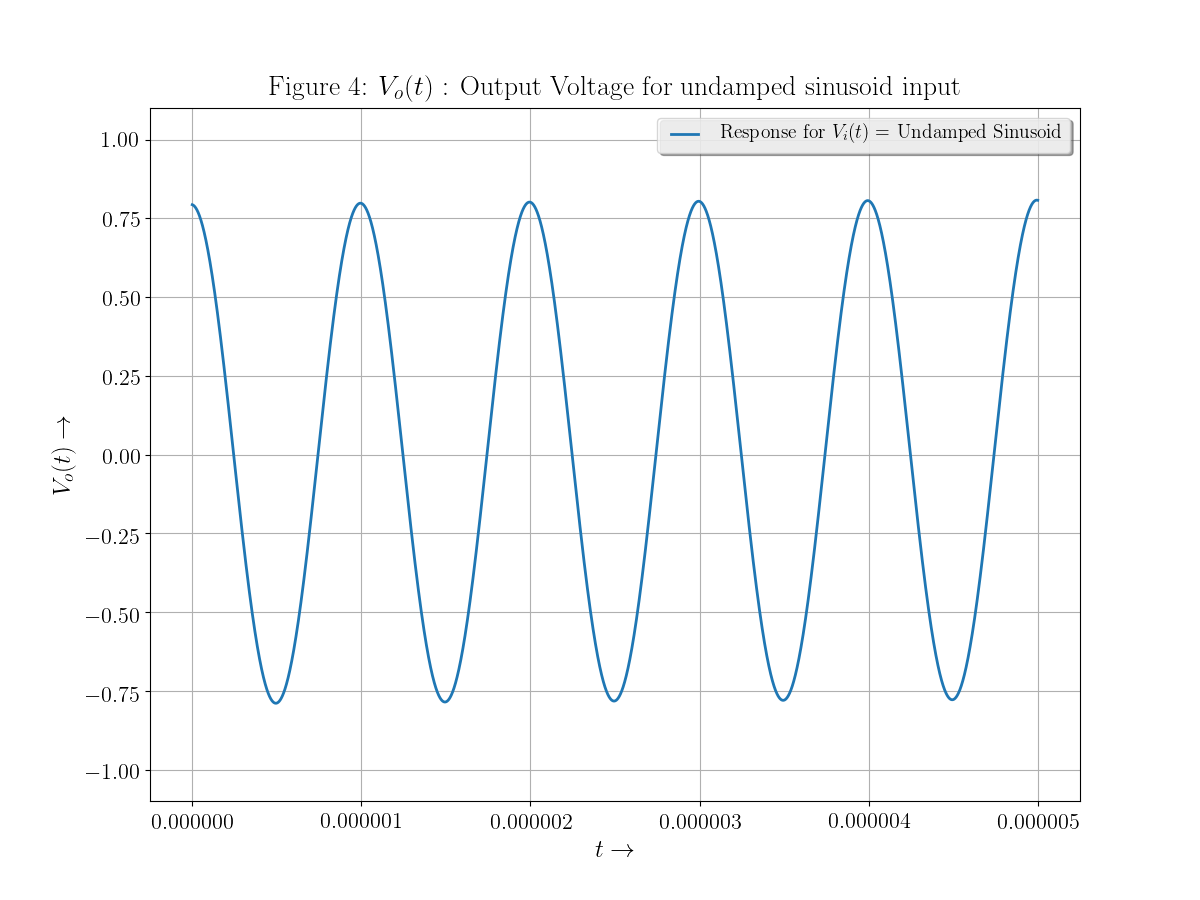
\includegraphics[scale=0.4]{./../Extras/A74.png}  % Mention the image name within the curly braces. Image should be in the same folder as the tex file. 
  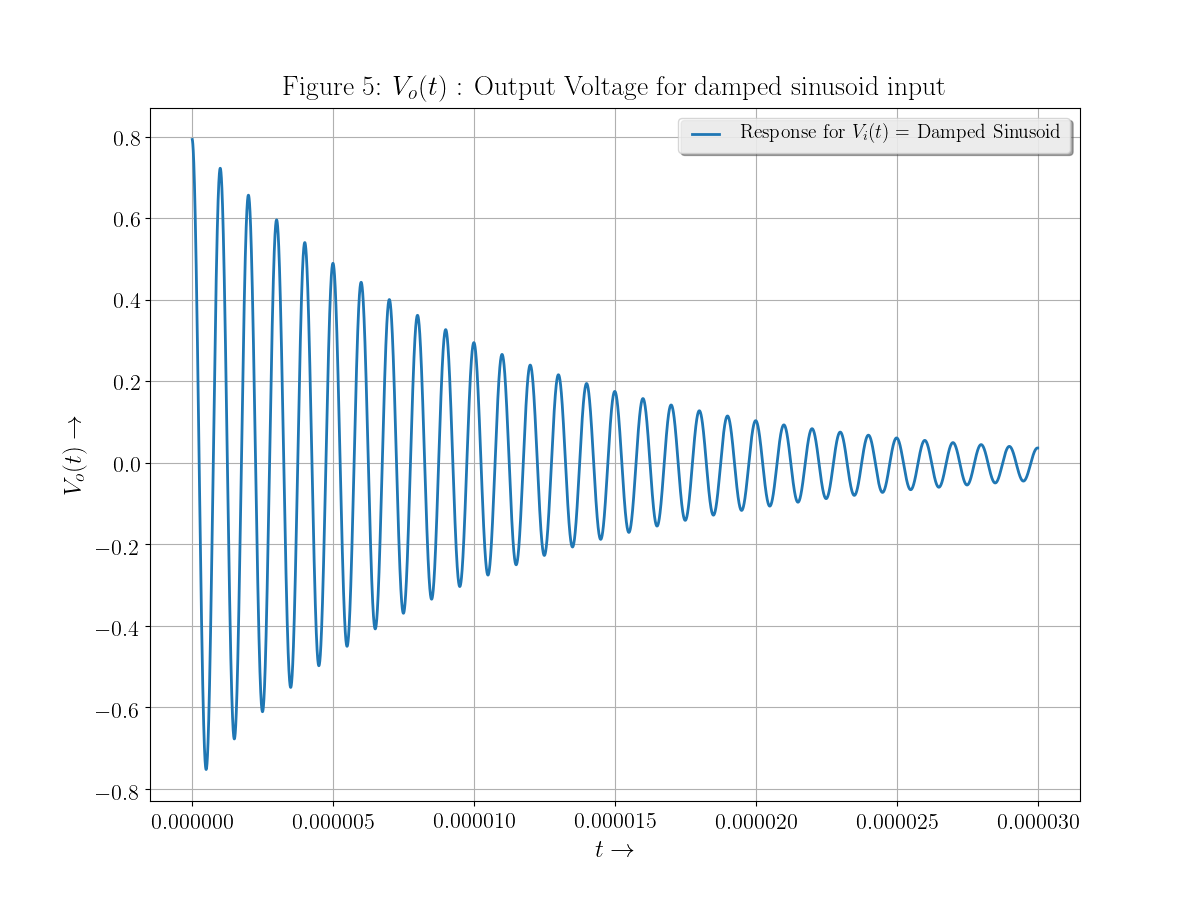
\includegraphics[scale=0.4]{./../Extras/A75.png}  % Mention the image name within the curly braces. Image should be in the same folder as the tex file. 
 
  \caption{Plots of sinusoid responses}
\end{figure}

\newpage
\subsubsection{Results and Discussion:}\label{results-and-discussion}

\begin{itemize}
  \item
  As we observe the plot and the circuit that we know it is a high pass
  filter with bandwidth $ \omega \textgreater{} 10^{5}$.
\item
  So the circuit will only pass input with frequencies which are in
  range of bandwidth only.
  \item
  As we observe the impulse response plot and the circuit that we know it is a high pass
  filter with bandwidth \\ \(\omega > 10^5\).

\item
  As we observe the step response plot that \(V_{o}(t)\) decreases quickly from 0.8 to
  0 and settles at 0 for after some time and remains constant.
\item
  But interestingly it \textbf{crosses zero and goes negative} for some
  period of time.
\item
  Because since the network is high pass filter, the output must not
  allow DC at steady state and since the input is unit step which is
  constant for \(t>0\) so at steady state \(V_{0}(t)\) should be zero.
  Also since its Highpass filter its \(Mean = 0\) which means
  \(\int_{0}^{\infty} V_{o}(t) dt = 0\).
\item
  So thats why we observe that the voltage becomes negative to make
  averge zero.
\item
  And we determined Quality factor of the system as
  \(Q = 0.453.. < \frac{1}{\sqrt{2}}\) Which implies that the gain of
  the system never exceeds DC Gain and always less than that. This
  observation comes by analysing the general form of second order
  transfer function.

\item
  Also If \(Q < 0.5\) system is overdamped since damping factor
  \(\zeta = \frac{1}{2Q} > 1\) for \(Q<0.5\) which means the unit step
  response will decrease slowly from 0.8 to \(0\) exponentially since
  its high pass filter and steady state voltage must be zero ,unlike
  immediately changing from \(0.8 \ to 0\)
\item
  So this is also observed in the plot as it slowly decays from 0.8 to 0
  and settles.
\item
  Also, we can see from the sinusoidal plots that only the frequency component 
  more than $10^{4}$ rad/s are passed through, thus we see both the damped and non-damped sinusoids have frequency of nearly $10^6$ rad/s, i.e. the cosine component
\end{itemize}
    \section{Conclusion :}\label{conclusion}

    \begin{itemize}

\item
  We successfully analysed circuits using laplace transform by solving
  analytically instead of numerical solutions using Symbolic python.
\end{itemize}


      
\end{document}